
\section{Methodology and Tools}
NOTES:
\begin{itemize}
\item Insist that everything in that section is my own work. It's not me citing
other people's work.
\item Description of how we implemented the model.
\end{itemize}



A large selection of tools exist to study laser-cluster interaction,
differentiating themselves through the amount of approximation taken.

Exact solution of the quantum mechanical system is, most of the time,
intractable. Theoretical investigations thus require some degree of
approximation, a compromise between feasibility and exactitude. On one end of
the spectrum, the most general methods is solving the
Time-Dependent \schrodinger Equation (TDSE) directly or the Quantum Monte-Carlo
(QMC) method. Unfortunately, these methods can only be applied to the simplest
systems of small numbers of electrons; clusters cannot be studied using these
methods.

Larger systems can be studied using \textit{ab initio} methods (``from
first principles'') which covers a wide range of techniques. In this class of
methods one can find \textit{Hartree-Fock} (HF) methods which consist on
approximating the ground state wavefunction by a single Slater determinant.
In HF methods, instantaneous electron-electron Coulomb repulsion is not
included directly in the system's Hamiltonian. Instead, only the average field
resulting from other electrons is used, giving the often used name of
\textit{self-consistent field} methods. Other \textit{ab
initio} methods are the \textit{Post Hartree-Fock} methods where electron
correlation is added. An example is the \textit{Configuration Interaction} (CI)
method. Because of their great accuracy, these methods are restricted to
relatively small systems, generally less then 10 atoms. Full \textit{ab initio}
treatment of clusters is not possible.

Larger systems requires more approximations. \textit{Density Functional Theory}
is an often used method for cluster studies requiring quantum aspects, with
either quantum or semiclassical propagation. It starts by formulating an
expression for the total energy of electrons and ions and derives static and
dynamic equations from it. All approximations are done in the selection of this
(energy) functional. The upper limit on these methods is of practical reasons,
mainly computational power available. On the other side, because the chosen
functional approximate the underlying quantum system, specific quantum effects
might not be included, for example shell effects or tunnelling are neglected.

Because DFT methods are mean field in nature, they cannot account for the large
field fluctuations seen in strong field cluster dynamics.

On the end of the methods spectrum lies the rate equations.






For a detailed review of the different methods, see Ref. \cite{Fennel2010}.





\subsection{Molecular Dynamics (MD)}
\label{section:tools:md}

Due to the high charge states seen in experiment with clusters the only
practical method to microscopically study the ionization dynamics is
\textit{Molecular Dynamics} (MD) methods where ions and electrons are treated
classically.

In MD, bodies interact directly through classical instantaneous forces. Even
though the method's name contains the term ``molecular'', these forces can be
of any nature; gravitational, van der Waals, Lennard-Jones, electrostatic, etc.
The method numerically integrates Newton's equations of motion, resulting in a
time evolution of the system.

The total force acting on particle $i$ of mass $m_i$ from all other $N$
particles in the system is:
\begin{align}
m_i \va_i & = \vF_i = \sum_{j \ne i} \vF_{j \rightarrow i}
\label{eqn:md:newton}
\end{align}
In the present work, the force between charged particles is the instantaneous
electrostatic Coulomb force:
\begin{align}
\vF_{C,j \rightarrow i}\pa{\vr} & =\frac{k q_i q_j}{r_{ji}^2} \hvr_{ji}.
\label{eqn:md:coulomb:F}
\end{align}
which only depends on the distance between particles. Figure
\ref{fig:md:vectors} shows the vectors definition used throughout this work. We
define particle $i$ the particle we are interested in (for example, the
particle we are calculating the force on), and particle $j$ the particle that
is generating the field or potential that is measured at location of particle
$i$. We thus have:
\begin{align}
\vr_{j} + \vr_{j,i} & = \vr_{i} \\
\vr_{j,i} & = \vr_{i} - \vr_{j}
\end{align}
%       _j
%       /|\
%  r_j /   \ r_ji
%     /    _\/
%    /------>i
%       r_i

\begin{figure}
 \centering
 
\includegraphics[width=0.5\columnwidth]{figures/vectors}
 \caption{\label{fig:md:vectors}Vectors definition between particles $i$ and $j$}
\end{figure}


Equation \eqref{eqn:md:newton} can be time integrated for every particles
$i$ using the Velocity-Verlet~(VV) scheme:
\begin{subequations}
\begin{align}
\vx_{i}^{\pa{n+1}} & = \vx_{i}^{\pa{n}} + \vv_{i}^{\pa{n}} \Delta t +
\frac{\va_{i}^{\pa{n}}}{2} \Delta t^2, \\
\va_{i}^{\pa{n+1}} & = \frac{\vF^{\pa{n}}}{m_i} \label{eqn:md:vv:a} \\
\vv_{i}^{\pa{n+1}} & = \vv_{i}^{\pa{n}} + \frac{\va_{i}^{\pa{n}} +
\va_{i}^{\pa{n+1}}}{2} \Delta t,
\end{align}
\label{eqn:md:vv}
\end{subequations}
where $\Delta t$ is the integration time step, $\vx_{i}$ the position vector,
$\vv_{i}$ the velocity vector and $\va_{i}$ the acceleration vector, all evaluated
for particle $i$ at either the time step $n$ or the next one $n+1$.
Equations \eqref{eqn:md:vv}, when applied to every particles $i$ of the system,
can thus be used to propagate in time the whole cluster. Note that some
variations of equations \eqref{eqn:md:vv} are possible but are equivalent.

Every particle in the system stores its position $\vx^{\pa{n}}$, its velocity
$\vv^{\pa{n}}$ and also the total force acting on it $\vF^{\pa{n}}$. This total
force is the sum of all contribution of equation \eqref{eqn:md:coulomb:F} from
all other particles in the system.

The MD algorithm basically calculates the force between every pair of particles
in the system. Since there is $N$ total particles, there is $O\pa{N^2}$
interactions to calculate. Doubling the number of particles will quadruple the
computational burden, effectively putting an upper limit on the number of
particles that can be simulated to tens of thousands.

An example cluster can be seen on figure \ref{fig:md:cluster}. A cluster
made of 147 xenon atoms (large blue spheres) absorbs some photons (red
wave-packets) from the laser field. Atoms are ionized; electron are created
(small grey spheres) which moves through the cluster. Ions are represented with
colours going from blue for neutral to red for Xe$^{5+}$. The figure was
generated using
PyMOL\footnote{\textit{The PyMOL Molecular Graphics System}, Version 1.5.0.4,
Schrödinger, LLC. \url{http://pymol.org/}}


\begin{figure}
 % set opaque_background, off
 \centering
 \includegraphics[width=\figurewidth]{figures/cluster}
 \caption{\label{fig:md:cluster}Example ionized Xe$_{147}$ cluster; xenon as
          large spheres with colours going from blue for neutral to full red for
          Xe$^{5+}$, electrons in small grey spheres. Photons from the laser
          field are displayed as red wave-packets.}
\end{figure}



\subsection{Short range potential: shapes}
\label{section:intro:md:potentials}

An important problem to consider is the close range behaviour of equation
\eqref{eqn:md:coulomb:F} which diverges. Additionally, electrons should not be
able to classically recombine to an ion under the atomic energy level. To
prevent the later, electron recombination, as described in section
\ref{section:intro:mechanisms}, can be enabled. But this does not prevent
the divergence of the Coulomb force at $r~=~0$. Instead, the problem is resolved by
changing the shape of equation \eqref{eqn:md:coulomb:F} at close range.
Different \textit{smoothing potentials} can be used to prevent the
discontinuity of the Coulomb potential (or force).


Different potential shapes were investigated for the close range potential.
Figure~\ref{fig:potential:shapes} plots the different shapes of potentials and
their respective electrostatic field. These shapes are obtained by simply
finding the location $R$ where the value and the slope of the close-range shape
$\phi_{cr}$ fits with the Coulomb potential $\phi_C$.
\begin{subequations}
\begin{align}
\left. \phi_C        \right|_{R} & = \left. \phi_{cr} \right|_{R} \\
\left. \delr{\phi_C} \right|_{R} & = \left. \delr{\phi_{cr}} \right|_{R}
\end{align}
\label{eqn:potential:to_match}
\end{subequations}

These locations $R$ are the cutoff radius of these shapes and mark the switch
between the long range Coulomb potential and the short range potential.


\subsubsection{Harmonic}

For the harmonic potential, we have:
\begin{align}
\phi_{j,H} & = -A r^2 + \phi_0
\end{align}
We note that at $r_{j,i} = 0$, the potential value is the ``potential depth''
$\phi_0$.
Matching equations \eqref{eqn:potential:to_match} at $R$ gives:
\begin{subequations}
\begin{align}
\phi_{j,H}\pa{\vr_i} & = \frac{-4 \phi_0^3}{27 \pa{k q_j}^2} r_{j,i}^2 + \phi_0
\\
R & = \frac{3 k q_j}{2 \phi_0} \\
\vE_{j,H}\pa{\vr_i} & = \frac{k q_j}{R^3} \vr_{j,i}
\end{align}
\end{subequations}


\subsubsection{Super-Gaussian}

The super-gaussian potential is given by:
\begin{align}
\phi_{j,SG}\pa{\vr_i} & = \phi_0 \ex{
                            -\frac{1}{2} \pa{\frac{r_{j,i}}{\sigma}}^{2m}
                        }
\label{eqn:potential:shapes:sg:pot}
\end{align}
In the case where $m = 1$, equation \ref{eqn:potential:shapes:sg:pot} is simply
a gaussian shape. Matching equations \eqref{eqn:potential:to_match} at $R$ gives
values for $\sigma$ and $R$:
\begin{subequations}
\begin{align}
\sigma  & = \frac{k q_j m^{1/2m}}{\phi_0} \ex{\frac{1}{2m}} \\
R       & = \frac{k q_j}{\phi_0} \ex{\frac{1}{2m}} \\
\vE_{j,SG} & = \frac{\phi_0 m}{r_{j,i}}
                \ex{-\frac{1}{2} \pa{\frac{r_{j,i}}{\sigma}}^{2m}}
                \pa{ \frac{r_{j,i}}{\sigma} }^{2m}
                \hvr_{j,i}
\end{align}
\label{eqn:potential:shapes:sg}
\end{subequations}





\subsubsection{Gaussian distribution}

An efficient way to correct the close range problem is to treat electrons as
charge distributions instead of point particles. There is thus no
discontinuity when the two charged distribution (particles) overlap. As such,
the electrostatic potential due to a charged particle $j$
(of gaussian shape of width $\sigma$) at location $\vr = r \hvr$ is:
\begin{align}
\phi_{j}\pa{\vr} & = \frac{k q_j}{r} \erf{\frac{r}{\sigma \sqrt{2}}}
\label{eqn:md:smoothed:phi}
\end{align}
The associated electrostatic field is thus:
\begin{align}
\vE_{j}\pa{\vr} & = -\grad{\phi_j\pa{\vr}} = k q_j \pa{
    \frac{ \erf{\frac{r}{\sigma\sqrt{2}}} }{r^2}
    - \sqrt{\frac{2}{\pi}} \frac{ \ex{-\frac{r^2}{2 \sigma^2}} }{\sigma r}
} \hvr
\label{eqn:md:smoothed:E}
\end{align}
When the distance $r$ is large compared to $\sigma$, the error function
is close to 1 and the potential becomes Coulombic. Also, the exponential
term in the electric field will tend towards 0 (since it's a gaussian shape).
The error function will tend towards 1, so the electric field will
be the field of a discrete point charge.

The value of $\sigma$ is arbitrary: the smaller it is, the closer the potential
will be from the pure Coulomb one. We can set a value for $\sigma$ from the
extremum value of the potential which occurs at $\vr = 0$. At $\vr = 0$, an
indetermination $\frac{0}{0}$ occurs. Using l'Hospital rule, we get the limit
of $\phi$ as $\vr$ reaches 0:
\begin{align}
\lim_{\vr \rightarrow 0} \phi_j\pa{\vr}
    & \equiv \phi_j\pa{0} = \frac{ k q_j }{ \sigma } \sqrt{\frac{2}{\pi}}
\end{align}
from which we get the particle width:
\begin{align}
\sigma & = \frac{ k q_j }{ \phi_j\pa{0} } \sqrt{ \frac{2}{\pi}}.
\label{eqn:md:sigma}
\end{align}
The free parameter is thus the ``potential depth'' $\phi_j\pa{0}$. Even
though $\phi_j\pa{0} > 0$ we call this parameter ``depth'' since the potential
energy of an electron on top of an ion would be minimum, similar to the
gravitational potential energy of a ball is minimum at the bottom of a well.

Another problem that the smoothing of equations \eqref{eqn:md:smoothed:phi} and
\eqref{eqn:md:smoothed:E} solve is the one of \textit{numerical heating} which
occurs when particles artificially gain (or loose) energy during the
calculation of equations \eqref{eqn:md:vv}. This absence of conservation of
energy is due to a time step $\Delta t$ which is too large. Indeed, the
discretization of equations \eqref{eqn:md:vv}, and most importantly of
subequation \eqref{eqn:md:vv:a}, assumes the force on each particle to have a
linear variation between time steps. If the time step is too large and the
curvature of equation \eqref{eqn:md:smoothed:E} cannot be sampled by the moving
particle between each time steps, then the energy will not be conserved.



Figure \ref{fig:potential:shapes} show the different potential shapes and their
respective electrostatic field.

\begin{figure}
 \centering
 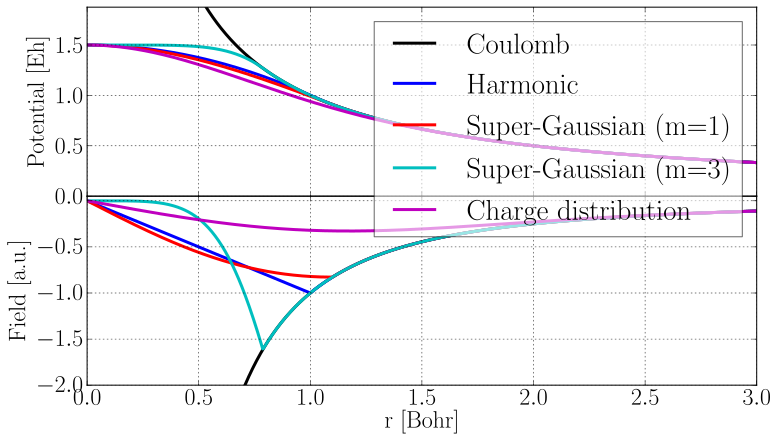
\includegraphics[width=\figurewidth]{figures/potential_shapes}
 \caption{\label{fig:potential:shapes}Potential shapes and their respective
          electric field. Note the use of atomic units and the potential depth
          $\phi_0$ = 1.5 Hartree = 40.8 eV.}
\end{figure}

It was found that the potential given by the charge distribution of equation
\eqref{eqn:md:smoothed:phi} and the associated electrostatic field of
\eqref{eqn:md:smoothed:E} give the less numerical heating. As explained
previously, the time discretization used to integrate the equations of motion
assume that the change in force between two time steps is linear. As can be
seen on figure \ref{fig:potential:shapes}, the charge distribution curve
(magenta) does not have a discontinuity and is therefore the prefered one.

To validate the selection of the smoothing curve, photo-ionization was forced
on a single atom and the total energy calculated. In this ionization case, the
electron comes out of the ion with a maximum of kinetic energy. It is thus a
good candidate to test if numerical heating is present or not. If the total
energy is conserved, then the selected parameters (potential depth, smoothing
curve and time step) can be used with good confidence. Figures
\ref{fig:potential:heating:dt} and \ref{fig:potential:heating:depth} show the
energy variation of the process as a function of time step (for different
potential depth) and as a function of potential depth (for different time step).
A time step of 0.5 as is often taken as, as can be seen on figure
\ref{fig:potential:heating:depth} it minimizes the energy variation for a large
range of potential depth. Additionally, it is still above the limit where
lowering the time step size does not reduce the error (around 0.05 as). This
limit is due to the floating point precision of the computer. The specific
parameters (time step and potential depth) are specified in the different
studies in later sections.


\begin{figure}
 \centering
 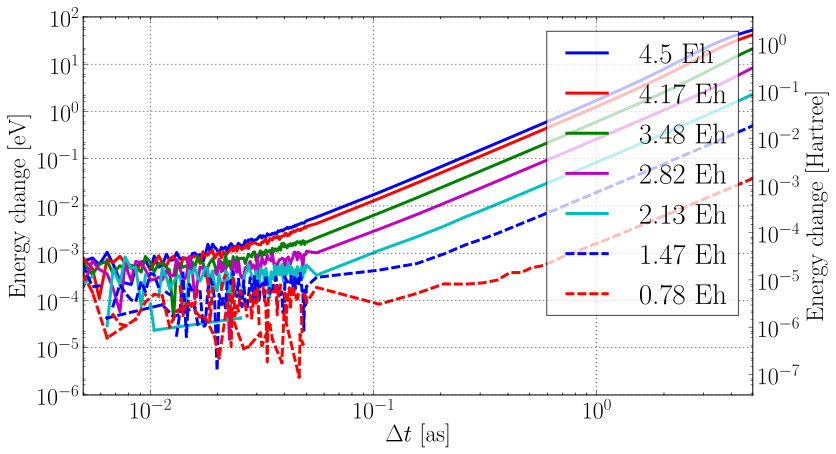
\includegraphics[width=\figurewidth]{figures/numerical_heating_dt}
 \caption{\label{fig:potential:heating:dt}Energy variation after single photon
          ionization as a function of the time step size $\Delta t$. Different
          potential depths used: 0.45 Eh (lowest curve), 1.1 Eh, 1.8 Eh, 2.5 Eh,
          3.15 Eh, 3.85 Eh and 4.5 Eh (highest curve)}
\end{figure}

\fxfatal[noinline,margin]{Remove the blue curve as it seems there is two!}
\begin{figure}
 \centering
 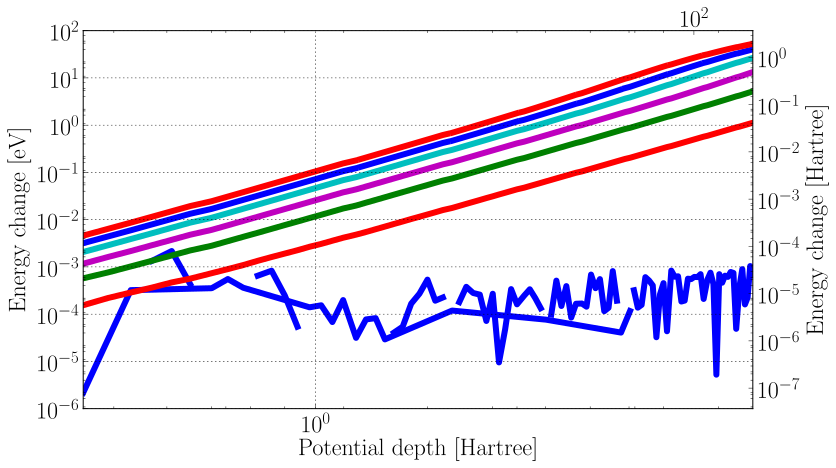
\includegraphics[width=\figurewidth]{figures/numerical_heating_D}
 \caption{\label{fig:potential:heating:depth}Energy variation after single photon
          ionization as a function of the potential depth. Different
          time step size used: 0.005 as (lowest curve), 0.8123 as, 1.67 as,
          2.477 as, 3.335 as, 4.1423 as and 5.0 as (highest curve)}
\end{figure}





\subsection{Long range potential: Hierarchical Tree algorithms}

The $O\pa{N^2}$ scaling of MD algorithm can be problematic when the number of
particles simulated is more than many thousands, which is a potential target
for laser-cluster interaction. Some interesting variations of the MD algorithm
exist to reduce the computational burden. These \textit{hierarchical tree}
algorithms were introduced\cite{Barnes1986} by Barnes and Hut in 1986. To
reduce the computational burden, particles are grouped in a hierarchical tree
(quadtree in two dimensions, octree in three). While Barnes used his
\textit{treecode} to solve the N-body problem in the context of gravitational
interactions, it can also be applied in the electrostatic case.

The main issue with the direct calculation of forces in MD is the lack of
distinction between the close particles and distant ones. While the resulting
potential of a distant particle is small, the computational cost required to
calculate it is the same as in the case of a nearby particle. Some MD
calculation use an artificial cutoff; particles farther then this cutoff will
be ignored in the calculation of the force on one particle. This is acceptable
when the force acting on particles is short range, either due to screening or
to the nature of the force. In the present work, the dominant force is the
Coulomb force and is a long range one by nature; it thus cannot be artificially
cutoff as in the case of close range forces used in other fields.

Could distant particles be grouped together, with their contribution to the
force (or potential) being calculated only once (per ``group'')? Because
individual particles which are part of a distant group will have a similar
contribution to the potential at the location of particle $i$, the interaction
with this group can be instead approximated through the multipole
expansion\cite{Gibbon2002} of the group of particles, or cell in terms of the
tree algorithm:
\begin{align}
\phi_i & = \sum_{j~\textrm{cell}} \phi_{j \rightarrow i} = \sum_{j~{\rm cell}}
\frac{k q_j}{r_{ji}} \\
& \approx \frac{M_{c}}{R}
+ \sum_{\alpha} \frac{r_{\alpha} D_{c,\alpha}}{R^3}
+ \frac{1}{2} \sum_{\alpha,\beta} \frac{
        Q_{c,\alpha,\beta} r_{\alpha} r_{\beta}
    }{R^5}
\end{align}
where $M_{c}$, $D_{c,\alpha}$ and $Q_{c,\alpha,\beta}$ are the monopole, dipole
and quadrupole moments of the cell defined as:
\begin{subequations}
\begin{align}
M_{c}           ~~~~& = \sum_{j~\textrm{cell}} q_{j} \\
D_{c,\alpha}      ~~& = \sum_{j~\textrm{cell}} q_{j} r_{j,\alpha} \\
Q_{c,\alpha,\beta}  & = \sum_{j~\textrm{cell}} q_{j} \pa{3 r_{j,\alpha}
r_{j,\beta} - r_{j}^2} \delta_{\alpha,\beta}
\end{align}
\label{eqn:tree:moments}
\end{subequations}
and $R$ is the distance between the cell's centre-of-charge and the
particle of interest $i$.

\fxwarning[margin,noinline]{The ``s'' variable is cut by the PDF}
\begin{figure}
 \centering
 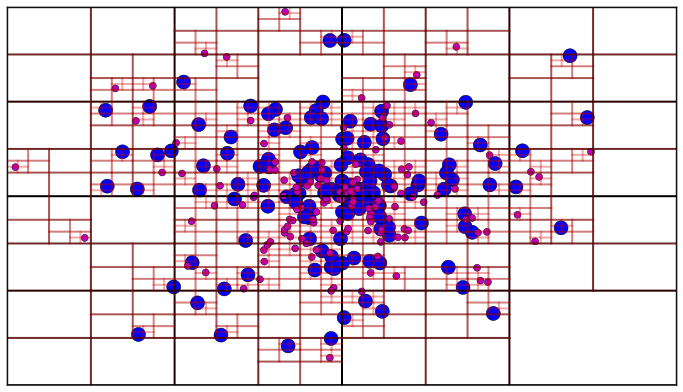
\includegraphics[width=\figurewidth]{figures/quadtree}
 \caption{\label{fig:tree:quadtree}Quadtree: 2D's equivalent of the 3D octree.
          300 particles (half ions in blue, half electrons in magenta) represent
          an exploding cluster. Cells' moments are propagated up the tree to the
          root cell. Particles far from a cell can interact directly with it
          instead of resolving all particles contained in it, thus reducing the
          computational burden.}
\end{figure}


The tree algorithm first split the computational domain into an octree (in
three dimension) or quadtree (in two dimensions) until
only a maximum of one particle is present per cell; see figure
\ref{fig:tree:quadtree}. The tips of the tree, containing only one particle,
are called leaves. Once every particles in the system are inserted in the tree,
the electrostatic moments are propagated from the leaves up to the root cell,
the top cell enclosing the whole domain.

Then, instead of iterating through all particles for the calculation of the
force on the particle of interest $i$, the tree is traversed. If the cell is
``far enough'' (with a given definition of far enough, discussed next) it can
be added to the a cell interaction list for later processing. In the case of
the cell being too close, it must be resolved into its  eight \textit{daughter}
cells (or four in 2D). The daughter cells containing particles are visited, while the empty
ones are ignored. The leaf cells can be reached using this process; in this
case, the particles in the leaves are considered close enough to the particle
of interest $i$ and a direct interaction is wanted. The leaf particle will thus
be added to a second interaction list containing particle-particle direct
interactions. The process is recursively repeated until all particles
are added to an interaction list, either directly or through a parent cell.
Note that an optimization done in the
implementation is to allow many particles per leaves and automatically add them
to the particles interaction list when traversing the tree, preventing trees
which are overly unbalanced.

Different selection rules exist for the criteria of ``far enough''. These
rules are called \textit{Multipole Acceptance Criteria} or
MAC\cite{Pfalzner1996}. Barnes' original one simply referred as
``\textit{s/d}'' compares an input parameter $\theta$ with the cell's size $s$
divided by the distance between the cell's center-of-charge and particle of
interest $i$. If the ratio $s/d$ is smaller than the parameter $\theta$, the
group of particles contained inside the cell is approximated through the cell's
moments and the cell is added to the cells interaction list. At the opposite, if
the ratio is larger than $\theta$, the cell will be resolved into its daughters.
In the limit where $\theta$ reaches zero, no more cells are added to the
cells interaction list (they are all resolved) and the MD algorithm emerges, though
with a large overhead due to the tree construction and traversal.

Unfortunately, this MAC can cause huge errors when large amount of charge is
present in a corner of a cell\cite{Pfalzner1996}.
% Page 85 (97), figure 4.13
In this case, a cell could be added to the cell
interaction list even though the error introduced by the multipole expansion is
significant. Different MAC have thus been proposed to mitigate this problem.
The \textit{minimum distance} MAC replaces the distance $d$ in the MAC with the
minimum distance to one of the cell's edge. The \textit{B-max} MAC instead
replaces the size of the cell with the largest distance between one of the
cell's corner to the center-of-charge. Another MAC was proposed by
B\'edorf~\textit{et.~al.}~\cite{Bedorf2012} and is a mix of the two previous.
The MAC reads:
\begin{align}
d > \frac{s}{\theta} + \delta
\end{align}
where $\delta$ is the distance between the cell's geometric center and its
center-of-charge. If the previous equation holds ($d$ is large enough) then the
multipole expansion is used; the cell is added to the interaction list.
The different MAC can be seen on figure \ref{fig:tree:mac}.

\begin{figure}
 \centering
    \begin{subfigure}{0.15\columnwidth}
        \centering
        \includegraphics[width=\textwidth]{figures/mac_1}
        \caption{ $s/d$}
        \label{fig:tree:mac:1}
    \end{subfigure}
    \hspace{0.75cm}
    \begin{subfigure}{0.15\columnwidth}
        \centering
        \includegraphics[width=\textwidth]{figures/mac_2}
        \caption{min. $d$}
        \label{fig:tree:mac:2}
    \end{subfigure}
    \hspace{0.75cm}
    \begin{subfigure}{0.15\columnwidth}
        \centering
        \includegraphics[width=\textwidth]{figures/mac_3}
        \caption{B-max}
        \label{fig:tree:mac:3}
    \end{subfigure}
    \hspace{0.75cm}
    \begin{subfigure}{0.15\columnwidth}
        \centering
        \includegraphics[width=\textwidth]{figures/mac_4}
        \caption{Bédorf\cite{Bedorf2012}}
        \label{fig:tree:mac:4}
    \end{subfigure}
\caption{Different Multipole Acceptance Criteria (MAC). See text for descriptions.}
\label{fig:tree:mac}
\end{figure}


Because not all interaction pairs are considered in the calculation of the
force and potential, a significant speedup is obtained. Due to the tree
traversal algorithm, the scaling passes\cite{Barnes1986,Gibbon2002,Pfalzner1996}
from $O\pa{N^2}$ to $O\pa{N \ln{N}}$; see figure \ref{fig:tree:scaling}.

\emptyfig{TREECODE SCALING}{fig:tree:scaling}
 \fxwarning[noinline,margin]{Create real figure: Tree scaling}

A variation to the hierarchical treecode is obtained when a sufficiently large
$\theta$ is used. In this case, the root cell (the largest one) is never
resolved into its daughters. By adding more moments to the approximation then
the first three ones of equations \eqref{eqn:tree:moments} and removing
contributions of nearby particles, the \textit{Fast Multipole Method} (FMM) is
obtained\cite{Pfalzner1996}. FMM was developed by Greegard in
1988\cite{Greengard1987} independently of Barnes' hierarchical tree method.
While conceptually similar, its implementation details are quite different and
has not been implemented in the current work.



\subsection{Implementation details}

Our group previously used Barnes and Hut treecode implementation,
freely available\cite{treecode} through the GPL version 2 license. The code was adapted
to simulate charged particles (Coulomb force) instead of masses (gravitational
force) with some ionization routines added (see for example reference
\cite{Jungreuthmayer2005}). While reducing development time by re-using already
written code, the maintenance burden introduced by many factors (initial
implementation written in the C language, usage of global variables
throughout the code, multiple coding styles from different people throughout
the years, lack of vision, lack of revision control system to give the freedom
of deleting code from the active version without loosing the ability to roll
back, many subtle and important bugs, stability issues, etc.) pushed me
to restart from scratch. This allowed using modern development techniques to be
used. For example, all development was done through a revision control system
(subversion\cite{svn} at first, then switched to git\cite{git}) in the C++
language instead of C. The object oriented nature of C++ allowed encapsulation
of different parts of the code which could then be tested and validated
individually. This gave better flexibility to the code, a required asset to
push further the development of features.

A substantial number of MD packages are freely available and
their usage was considered instead of re-implementing a new one from scratch.
Examples are GROMACS\footnote{GROMACS:
\url{http://www.gromacs.org/}}, NAMD\footnote{NAMD:
\url{http://www.ks.uiuc.edu/Research/namd/}} and
LAMMPS\footnote{\url{http://lammps.sandia.gov/}}. A major issue with these
pre-existing MD packages is their target audience; they aim to simulate large
bio-molecules with mostly short range interactions. Another important problem
is the number of particles throughout the simulations; while many packages
assume a constant number of particles, the present work required creating
(ionization) and annihilating (recombination) particles throughout simulations.
Controlling the MD part of the code allowed better integration of the
ionization aspects.

Additionally, other MD packages were not mature enough or simply non-existent at the time.
For example the largely used HOOMD-blue\footnote{HOOMD-blue:
\url{http://codeblue.umich.edu/hoomd-blue/}} which uses extensively
Nvidia GPUs released its first version (v0.6.0) in February 2008.
Additionally, the knowledge and experience gained by writing from scratch such
a package is invaluable.


\subsubsection{Potential threshold $V_b$}
\label{section:intro:Vb}

Many ionization processes described previously consider an isolated atom but
clusters have close to solid density (10$^{22}$ -- 10$^{23}$ cm$^{-3}$) and
so the environment cannot be ignored.

The cluster environment can be approximated by a constant value that shifts the
potential\cite{Fennel2007}. This shift $U_b = -e_0 V_b$ where $V_b$ is the
potential due to the cluster at the ion's location (ignoring nearby electrons)
and $U_b$ is the potential energy a test particle of charge state -1 (an electron)
would have if it was placed right on top of the ion. This can be justified by
the fact that bound states of rare gas atoms are localized close to the atoms
and the cluster potential spatial variation around atoms is small.

To illustrate this shifting, figure \ref{fig:md:Vb} shows the potential energy
landscape of an example ``cluster'' of two ions. Plotted on this figure is the
potential energy of a test particle of charge state -1 (an electron) in the
cluster environment. Note the distinction between potential and potential
energy. A positive charge (an ion) creates a positive potential but the
potential \textit{energy} of the test particle (of charge state -1) in that
positive potential is negative, hence the negative curves on figure
\ref{fig:md:Vb}. The contribution from the ion is the blue dashed line on the
figure.



\begin{figure}
    % ./potential_landscape.py --two --ion="0,1" --ion="-15,5" --impe_r=4 \
    %     --depth=1.5 --ion_impe=0 --impe_K=0.75 --ionization --umin=-1.2 \
    %     --umax=0.3 --plot=all --rmin=-7 --rmax=7.5 --plot=U
    \begin{center}
    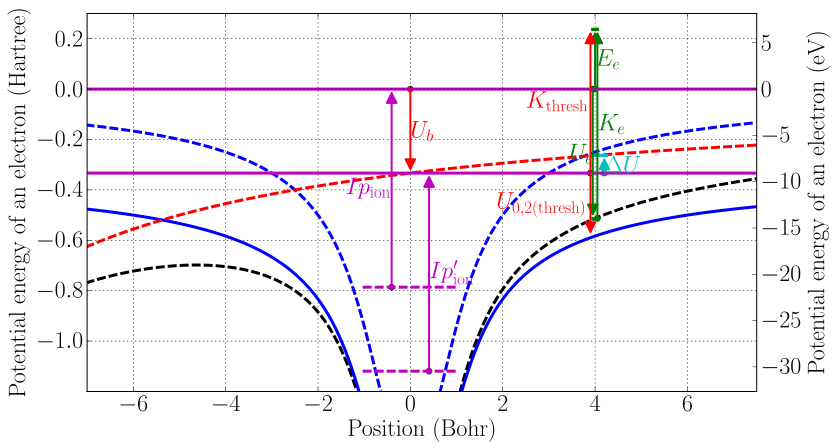
\includegraphics[width=\figurewidth]{figures/potential_landscape}
    \end{center}
    \caption{\label{fig:md:Vb}Cluster environment potential energy landscape
             and the $U_b$ approximation. A 1+ ion at $r=0$ and a 5+ at
             $r=-15$~Bohr. The potential energy curves are those of a test
             particle of charge state -1 (electron). See text for curves
             description.}
\end{figure}


Continuing in the example case of figure \ref{fig:md:Vb}, we introduce a
second ion that will simulate the cluster environment. This second ion, of
charge state 5+ and located at $r$~=~-15 Bohr, is creating a
potential that is not constant around the first ion. The potential energy of
the test particle in this potential is plotted as the red dashed line. The total
potential energy of the test particle due to the two ions is plotted as a black
dashed line.

The first ion's threshold is thus influenced by the second ion. The continuum,
instead of being at zero, is shifted by $U_b$. This approximates the
influence of the second ion as being constant in the first ion's vicinity. This
threshold shift is shown on figure \ref{fig:md:Vb} as the red arrow $U_b$.

The effect of $U_b$ is to shift the ion's states to lower energies. This is
shown on the figure as $Ip_{ion}$, the energy required for a bound electron
to be promoted to the isolated ion's continuum, being shifted downward to
$Ip_{ion}'$. The effective ion's potential energy curve, also shifted by $U_b$,
is shown as the dotted blue line.

When an electron enters the picture, for example during collisional ionization
or ACI, atomic properties of isolated ions are used. These properties require
impacting electrons to come from infinity where the electron does not feel the
ion at all. At infinity, the electron's total energy only contains kinetic
energy. We call this kinetic energy $K_{\textrm{thresh}}$ for ``kinetic energy
above the threshold''. This $K_{\textrm{thresh}}$ can simply be calculated, in
an isolated system, as $K_{\textrm{thresh}} = K_e + U_e$ where $K_e$ is the
electron's kinetic energy and $U_e$ its potential energy; $K_{\textrm{thresh}}$
is, in this case, basically the electron's total energy. $K_{\textrm{thresh}}$
is the kinetic energy that must be used in Lotz formula
\eqref{eqn:impact:ionization:lotz}. Note that, contrary to a real kinetic
energy, $K_{\textrm{thresh}}$ can be negative. In that case, a null value is
used instead.

When a cluster environment is present, a similar approach is taken to obtain
$K_{\textrm{thresh}}$. Instead of taking the extra energy above zero for
$K_{\textrm{thresh}}$, the extra energy above the new threshold $U_b$ is used.
This value can easily be obtained from the actual electron's kinetic energy
$K_e$, it's \textit{total} potential energy in the cluster environment and the
threshold $U_b$ by:
\begin{align}
K_{\textrm{thresh}} & = K_e - \pa{U_b - U_e}.
\label{eqn:md:kthresh}
\end{align}
Again, $K_{\textrm{thresh}}$ could end up negative. In that case, zero is used
instead. $K_{\textrm{thresh}}$ is shown on figure \ref{fig:md:Vb} as a red arrow
with its base at $U_b$.

This cluster potential $U_b$ is then treated at the atom's threshold
to continuum. By using $U_b$ as the threshold, atomic properties such as
impact ionization cross-sections can be used, even in the cluster environment.



\subsubsection{Notes on ionization definition}
\label{section:intro:mechanisms:notes}
Special care needs to be taken when calculating particle energies during
ionization processes. In this work, an ionization event is defined as one
electron that leaves its parent ion, reaching infinity with a final kinetic
energy of zero.


\subsubsubsection{Single photon ionization}

In the case of single photon ionization of an isolated atom, when the electron
reaches infinity it will have, as its kinetic energy, the difference of energy
between the absorbed photon and the ionization potential of the ion.


\subsubsubsection{Impact ionization}

For impact ionization, the impacting electron's kinetic energy used in equation
\eqref{eqn:impact:ionization:lotz} is the kinetic energy the electron has
\textit{at infinity}, meaning that the impacting electron and the atom (or ion)
are isolated from each other. We change that definition to \textit{above
threshold}: in the case of an isolated atom, the threshold is at zero, but in the
case of a cluster environment, the threshold is taken as $U_b$, as described in
section \ref{section:intro:Vb}. If the impacting electron has more kinetic
energy, it can either keep the extra, give all the extra, or give a fraction of
the extra to the new electron. We split the extra kinetic energy between the two
electrons to assure that they do not fall back unto the ion.


Figure \ref{fig:impact:before:Z} shows the process of impact ionization when an
electron (particle 1) of charge state -1 impacts an ion (particle 0) of charge
state Z and creates a new electron (particle 2) right on top.

\begin{figure}
 \centering
    \begin{subfigure}{0.48\columnwidth}
        \centering
        \includegraphics[width=\textwidth]{figures/impact_ionization_t00}
        \caption{Before impact ionization (Z)}
        \label{fig:impact:before:Z}
    \end{subfigure}
\\
    \begin{subfigure}{0.48\columnwidth}
        \centering
        
\includegraphics[width=\textwidth]{figures/impact_ionization_t0}
        \caption{During impact ionization (Z+1)}
        \label{fig:impact:before:Zp1}
    \end{subfigure}
%
    \begin{subfigure}{0.48\columnwidth}
        \centering
        \includegraphics[width=\textwidth]{figures/impact_ionization_t1}
        \caption{After impact ionization}
        \label{fig:impact:after}
    \end{subfigure}
\caption{Impact ionization: before and after}
\label{fig:impact:steps}
\end{figure}


First, let's assume the impacting electron came from infinity where it's kinetic
energy was exactly the Ip. In that case, impact ionization will occur (considering
its impact parameter lies inside the cross-section). By definition, we must have two
electrons leaving to infinity: an unbound system. Such an unbound system has a total
energy of 0.

The total energy before (a) is thus:
\begin{align}
E^{a} & = K_{1}^{a} + U_{01}^{a} = Ip
\label{eqn:Ea}
\end{align}
and after (c) ionization is:
\begin{align}
E^{c} & = K_{1}^{c} + K_{2}^{c} + U_{01}^{c} + U_{02}^{c} + U_{12}^{c} = 0
\label{eqn:Ec}
\end{align}

The change in energy is thus:
\begin{align}
E^{a} - E^{c} & = Ip = K_{1}^{a} + U_{01}^{a} - \pa{
    K_{1}^{c} + K_{2}^{c} + U_{01}^{c} + U_{02}^{c} + U_{12}^{c}
}
\end{align}

The only unknown values here are $K_{1}^{c}$ and $K_{2}^{c}$ since the new electron is
created right on top of the ion. Let's isolate the final kinetic energies:
\begin{align}
K_{1}^{c} + K_{2}^{c} = K_{1}^{a} + U_{01}^{a} - \pa{
    U_{01}^{c} + U_{02}^{c} + U_{12}^{c}
} - Ip
\label{eqn:K1cPlusK2c}
\end{align}

We have a single constraint from equation \eqref{eqn:K1cPlusK2c} but two unknown. We thus
give an arbitrary value to one of the two. We want the new electron to leave the ion.
Since it is right on top of it, we can guess the required kinetic energy to be very close
to (minus) the potential energy the electron has with respect to the ion. But this electron
will be ``pushed'' be the impacting electron too and will thus be accelerated. To compensate
for this push, we remove the potential energy between the two electrons from the new electron's
kinetic energy. So the educated guess for the final kinetic energy of the new electron is:
\begin{align}
K_{2}^{c} & = -U_{02}^{c} - U_{12}^{c}
\label{eqn:K2c:pushed}
\end{align}

Using equation \eqref{eqn:K2c:pushed} in equation \eqref{eqn:K1cPlusK2c} gives:
\begin{align}
K_{1}^{c}
 & = K_{1}^{a} + U_{01}^{a} - \pa{
    U_{01}^{c} + U_{02}^{c} + U_{12}^{c}
} - Ip - K_{2}^{c} \\
 & = K_{1}^{a} + U_{01}^{a} - \pa{
    U_{01}^{c} + \cancel{ U_{02}^{c} } + \bcancel{ U_{12}^{c} }
} - Ip + \cancel{ U_{02}^{c} } + \bcancel{ U_{12}^{c} } \\
K_{1}^{c}
 & = K_{1}^{a} + U_{01}^{a} - U_{01}^{c} - Ip
\label{eqn:K1c:pushed}
\end{align}

The final total energy is then:
\begin{align}
E^{c}
 & = \pa{
    K_{1}^{a} + U_{01}^{a} - \cancel{ U_{01}^{c} } - Ip
 } - \pa{
                 \cancel{ U_{02}^{c} } + \bcancel{ U_{12}^{c} }
} + \cancel{ U_{01}^{c} } + \cancel{ U_{02}^{c} } + \bcancel{ U_{12}^{c} } \\
 & = K_{1}^{a} + U_{01}^{a} - Ip \\
 & = Ip - Ip \\
E^{c} & = 0
\end{align}
which is what was expected.






% Additionally, momentum is conserved by giving the two leaving electrons an angle
% of divergence. Since the impacting electron can cause ionization before being
% exactly on top of the atom or ion, the angle of divergence is given by:
%
% Figure \ref{fig:impact:direction} shows the convention of the two angles $\theta$ and $\phi$.
%
% \begin{figure}
% \begin{center}
% \includegraphics[width=0.8\textwidth]{figures/impact_ionization_directions}
% \end{center}
% \caption{Impact ionization: Direction for electrons}
% \label{fig:impact:direction}
% \end{figure}
%
%
% Momentum is conserved in each dimension. In this case, it's a 2-D plane.
% \begin{align}
% \vp^{a} & = \vp^{c} \\
% \vp^{a} & = m_e v_{1x}^{a} \hat{x} \\
% \vp^{c} & = m_e \pa{v_{1x}^{c} + v_{2x}^{c}} \hat{x} + m_e \pa{v_{1y}^{c} + v_{2y}^{c}} \hat{y}
% \end{align}
% with:
% \begin{subequations}
% \begin{align}
% v_{1x}^{a} & =  v_{1}^{a} \\
% v_{1x}^{c} & =  v_{1}^{c} \cosine{\theta} \\
% v_{2x}^{c} & =  v_{2}^{c} \cosine{\phi} \\
% v_{1y}^{c} & =  v_{1}^{c} \sine{\theta} \\
% v_{2y}^{c} & = -v_{2}^{c} \sine{\phi}
% \end{align}
% \end{subequations}
%
% Conservation in $x$:
% \begin{align}
% v_{1x}^{a}      & = v_{1x}^{c} + v_{2x}^{c} \\
% v_{1}^{a}       & = v_{1}^{c} \cosine{\theta} + v_{2}^{c} \cosine{\phi} \\
% \cosine{\phi}   & = \frac{v_{1}^{a} - v_{1}^{c} \cosine{\theta}}{v_{2}^{c}}
% \label{eqn:cos_phi}
% \end{align}
% and in $y$:
% \begin{align}
% 0           & = v_{1y}^{c} + v_{2y}^{c} \\
% 0           & = v_{1}^{c} \sine{\theta} - v_{2}^{c} \sine{\phi} \\
% \sine{\phi} & = \frac{v_{1}^{c}}{v_{2}^{c}} \sine{\theta}
% \label{eqn:sin_phi}
%  % \\
% % \phi        & = \asin{ \frac{v_{1}^{c}}{v_{2}^{c}} \sine{\theta} }
% \end{align}
%
% Squaring and summing \eqref{eqn:cos_phi} and \eqref{eqn:sin_phi} gives 1:
% \begin{align}
% 1
% & = \cossquared{\phi} + \sinsquared{\phi} \\
% & = \pa{ \frac{v_{1}^{a} - v_{1}^{c} \cosine{\theta}}{v_{2}^{c}} }^2
%   + \pa{ \frac{v_{1}^{c}}{v_{2}^{c}} \sine{\theta} }^{2} \\
% \pa{ v_{2}^{c} }^2
% & = \pa{ v_{1}^{a} - v_{1}^{c} \cosine{\theta} }^2
%   + \pa{ v_{1}^{c} \sine{\theta} }^{2} \\
% & = \pa{ v_{1}^{a} }^{2} + \pa{ v_{1}^{c} }^{2} \cossquared{\theta}
%     - 2 v_{1}^{a} v_{1}^{c} \cosine{\theta}
%     + \pa{ v_{1}^{c} }^{2} \sinsquared{\theta} \\
% & =   \pa{ v_{1}^{c} }^{2} \underbrace{\pa{ \cossquared{\theta} + \sinsquared{\theta} }}_{=1}
%     + \pa{ v_{1}^{a} }^{2}
%     - 2 v_{1}^{a} v_{1}^{c} \cosine{\theta} \\
% \pa{ v_{2}^{c} }^2
% & =   \pa{ v_{1}^{c} }^{2}
%     + \pa{ v_{1}^{a} }^{2}
%     - 2 v_{1}^{a} v_{1}^{c} \cosine{\theta} \\
% 2 v_{1}^{a} v_{1}^{c} \cosine{\theta}
% & =   \pa{ v_{1}^{c} }^{2}
%     + \pa{ v_{1}^{a} }^{2}
%     - \pa{ v_{2}^{c} }^2 \\
% \cosine{\theta}
% & = \frac{
%       \pa{ v_{1}^{a} }^{2}
%     + \pa{ v_{1}^{c} }^{2}
%     - \pa{ v_{2}^{c} }^2
%     }{ 2 v_{1}^{a} v_{1}^{c} }
% \label{eqn:cos_theta}
% \end{align}
%
% Equation \eqref{eqn:cos_theta} is used to get $\theta$ from $v_{1}^{a}$ (initial velocity of
% the impacting electron), $v_{1}^{c}$ (final velocity of the impacting electron) and
% $v_{2}^{c}$ (final velocity of new electron). Once the angle $\theta$ is found, $\phi$ can
% be found using \eqref{eqn:cos_phi}.
%



\subsubsection{Cross-sections}
\label{section:intro:md:cross-sections}

Implementing any kind of ionization in the model is done through cross-sections.
Because cross-sections can be obtained from experiments for any kind of target,
it is easily integrated into the model.


\subsubsubsection{Single photon ionization}

For single-photon ionization, experimental cross-sections $\sigma\pa{\omega}$
for Xenon were obtained from reference \cite{West1978} and from
reference \cite{Marr1976} for Argon.

Once cross-sections are obtained, they are converted to a rate of ionization
using
\begin{align}
\Gamma\pa{\omega} = \sigma\pa{\omega} I\pa{t}.
\label{eqn:ionization:rate:single}
\end{align}
which is equivalent to equation \eqref{eqn:ionization:rate:mpi} with $\nu = 1$.

Then, this rate is weighted\cite{Lax2006} by the time step size and compared to
a random number $r$ between 0 and 1:
\begin{align}
1 - \e{-\Gamma \Delta t} > r
\label{eqn:ionization:prob}
\end{align}
When the previous test succeeds, ionization takes place and a new electron is
created in the code.

Using equation \eqref{eqn:ionization:prob}, a choice is made. If ionization is
to take place, the new electron is created right on top of the ion with a
kinetic energy set as the difference between the ionization potential and the
photon energy \textit{plus} the absolute value of the potential energy of the
electron with respect to its parent ion (with updated charge). This assure that
the electron that leaves the ion will reach infinity with a kinetic energy being
the difference between the Ip and the photon energy.
Then, the intensity profile of the laser $I\pa{t}$ is decreased
by one photon for better description of low fluence pulses.


\subsubsubsection{Collisional processes}

For impact ionization cross-sections, Lotz formula of equation
\eqref{eqn:impact:ionization:lotz} is used with experimental parameters obtained
from reference \cite{Tawara1987} (for neutral xenon) and \cite{Heidenreich2005}
(for higher charge states). For argon, data from \cite{Lotz1967} and
\cite{Lotz1970} is used.

As for ACI, numerical cross-sections from ground state to excited state and from
excited state to continuum were calculated by Edward Ackad using a
Hartree-Fock code from \cite{CowanCode}. Only the first eight excited states
were considered (with $l<4$) for charge states up to 17+ for both xenon and argon.

The impact parameter of the impacting electron is calculated by:
\begin{align}
b & = \frac{\abs{\vv \times \vr}}{\abs{\vv}}
\label{eqn:ionization:impact:parameter}
\end{align}
where $\vv$ is the impacting electron's velocity vector and $\vr$ the vector
from the impacting electron to the target. If the impacting parameter lies
inside the calculated cross section, excitation or ionization takes place. In
the case of excitation, the total cross-section of all excited states are used
and a final state randomly selected between all accessible, weighted by their
cross-sections relative to the total one.


% http://en.wikipedia.org/wiki/Neutron_cross_section#Link_to_reaction_rate_and_interpretation

\subsubsection{Recombination}

In a classical simulation electrons could cool down into ions' infinite Coulomb
potential where they would have a total energy less then what is allowed
according to quantum mechanics. Recombination is thus used to prevent such
unphysical events.

Additionally, recombination plays an important role in the dynamics of the
exploding cluster. Experiments at FLASH in 2009 on Xenon clusters in the XUV
regime\cite{Thomas2009} could be reproduced by our models when recombination
was enable; we found that the lower charge states detected would come from the
cluster core where recombination is important. This study is to be published in
May 2013's edition of New Journal of
Physics\footnote{\url{http://iopscience.iop.org/1367-2630/page/Forthcoming\%20articles}}.

Recombination was also included in the fifth study, included in section
\ref{section:papers:100nm}, as it allowed to lower the potential depth of the
ions for more physical simulations.

Recombination is tested by calculating the total energy of an electron and
comparing it to the threshold $U_b$ -- see figure \ref{fig:md:Vb}. If
the energy is less then $U_b$, the electron is recombined; the ion charge is
decremented and the electron is removed from the ion. The electron's momentum
is transferred to the ion.\fxnote[margin,noinline]{Is the momentum really
transferred to the ion during recomb.?}


\input{introduction_qfdtd.tex}
\subsection{Acceleration through OpenCL and GP-GPUs}
A new trend lately in High Performance Computing (HPC) is code acceleration
through graphics cards. Similar to the ubiquitous Moore's Law in the CPU world,
video cards power evolved exponentially during the last twenty years, pushed
by the never ending need of more realistic video games. From ``dumb'' devices
drawing primitive shapes on a display, they evolved to extremely powerful
devices and started to act more like CPU by being programmable (shaders) during
the first half of 2000. The term \textit{Graphical Processing Unit} (GPU) was
coined in 1999 by Nvidia, the biggest vendor of video cards, as a selling point
to their product and to emphasize the fact that their chips were becoming more
and more alike CPUs.

Due to this increase in power, people tried to use these video cards as
accelerators for other things than real video operations. Because GPUs have
intrinsically high parallelism (for example the same operation is performed on
all pixels of an image in parallel) HPC users and developers got interested.
In his 2005 book, Taflove described a way to use a video card's GPU to
accelerate his electrodynamics FDTD solver \cite{Taflove2005}. At that time no
General-Programming GPU (GP-GPU) framework existed so Taflove (and anyone
interested in using GPUs at that time) had to ``translate'' the FDTD algorithm
into one that could be understood by a video card. This process was extremely
hard as it required using low level graphic primitives; in his case, OpenGL
calls. Normally OpenGL is used to draw animated scenes on the user's screen.
Notable examples of OpenGL usage is video games where the user is immersed in a
virtual three dimensional space. The process of re-writing an algorithm into
OpenGL calls is one that only a few highly skilled and knowledgeable people can
tackle.

In 2007, Nvidia saw an opportunity for market expansion. Why not let
non-videogames programmer use the powerful GPUs for something else then video
operations? For this to happen, a programming framework had to be released; the
amount of programmers and scientists able to exploit OpenGL to their advantage
was limited. They thus released their \textit{Compute Unified Device
Architecture} (CUDA), later just renamed CUDA. CUDA allows writing normal C or
C++ programs with some extensions, called \textit{kernels}, that can be run on
the GPU. These kernels have the same structure as C functions but are executed
concurrently by every cores on the GPU\footnote{Technically, GPUs don't have
``cores'' \textit{per se} like CPUs but the comparison can still be made.}. The
number of cores on a recent consumer grade video card is now of the order of
many hundreds; a 50\$ Nvidia GT 620 has 96 CUDA cores and 1 GB of RAM, while the
GTX TITAN has 2688 CUDA cores and 6 GB but cost more than 1,000 \$. Even though
the highest priced GPU can be more expensive than complete workstations, no CPUs
can offer close to three thousand cores for a still affordable price.

A year after CUDA was released, Apple wanted a framework that would allow
programs to be accelerated on their top-of-the-line product's GPU while still
being able to run on their lower-end range of products (which did not have a
discrete video card). Additionally, some Apple products were released with ATI
video cards (Nvidia's main competitor) which, understandably, never supported
CUDA. They thus released a framework called \textit{OpenCL} (standing for
Open Compute Language) in 2008 with the help of many partners (IBM, ATI, Intel
and even Nvidia). While conceptually similar to CUDA (smaller routines are
written in a kernel function and launched individually on the GPUs by the main
program) OpenCL has the advantage of targeting heterogeneous platforms
consisting of (possibly and not limited to) many CPUs, many cores and GPUs. The
main advantage of OpenCL is its portability; a program written in OpenCL can
not only run on GPUs from ATI and Nvidia but also on traditional CPUs,
exploiting all cores available on the CPUs transparently.

It was thus decided to port the two codes (MD and QFDTD) to OpenCL to take
advantage of the GPU power while retaining portability.

Some things are important to consider when porting codes to GPU frameworks.
First, because a core on a GPU is quite slower than a core on a CPU,
parallelisms must be extracted from algorithms. Second, the main drawback of
GP-GPU programming is the fact that GPUs have their own memory, independent of
the system's memory; kernels will only have access to the device's memory. Data
required for kernel calculation must thus be first transferred to the device's
memory and similarly the resulting data must be transferred back to the host
memory where it can be further processed by the rest of the main program. Video
cards today are connected to a computer through PCI-Express (PCIe) connections.
While fast, it can still be a bottleneck if data is to be transferred back and
forth similarly to main memory. It is thus necessary to reduce to a minimum the
data transfer between the host and the device, similarly to communications in a
distributed memory parallel programming paradigm.

In the case of the MD algorithm, every interaction pair is independent of all
others and can thus be calculated concurrently; this is the basis of the
OpenCL implementation. The main loop that calculates the electrostatic field
and potential at every particle's position is implemented as an OpenCL kernel.
Each thread on the GPU will thus calculate the interaction between one particle
and all others. Once the MD kernels are launched on the GPU, they are only
halted when either ionization is to be calculated (every femtosecond) or
when data needs to be saved (to take a snapshot of the simulation for example).
This prevent the GPU from being interrupted too often and reduces the amount of
data transfers. Using this OpenCL implementation, MD simulations could be run
80 times faster than on conventional CPUs.

As for the QFDTD, only the real time algorithm was implemented as OpenCL
kernels since the imaginary time method did not require long simulation times.
As in the case of the MD, the real time algorithm is left running on the GPU
until data needs to be saved to a snapshot or post-processed to reduce
transfers.


\subsection{Libraries}

Additionally to the MD and QFDTD packages, eight libraries were developed to
support some generic features shared between the two. These libraries are:
\begin{itemize}
\item timing.git\footnote{ \url{
    https://gitlab.cphoton.science.uottawa.ca/nbigaouette/timing}}:
    Timing routines used to measure running time, estimated time of arrival
    (ETA), code profiling, etc.
\item stdcout.git\footnote{ \url{
    https://gitlab.cphoton.science.uottawa.ca/nbigaouette/stdcout}}:
    Logging features allowing saving the output of any simulations to a
    (compressed) log file.
\item prng.git\footnote{ \url{
    https://gitlab.cphoton.science.uottawa.ca/nbigaouette/prng}}:
    Pseudo-random number generator (PRNG) library. Wrapper around
    dSFMT\cite{prng2009}, a SIMD-oriented Fast Mersenne Twister implementation.
    Defines easy to use PRNG functions, distributions, seed, etc. Keeps track of
    the seed and how many times pseudo-random numbers were generated, allowing
    to replay the series in case of simulation reloading.
\item memory.git\footnote{ \url{
    https://gitlab.cphoton.science.uottawa.ca/nbigaouette/memory}}:
    Wrappers around malloc() and calloc() that will automatically check that
    the allocation succeeded. Will also keep track of the amount of
    memory allocated and allow setting a maximum value, preventing
    over-allocation due to bugs or user errors. Can also return the binary
    representation of a number as a string for easier debugging.
\item io.git\footnote{ \url{
    https://gitlab.cphoton.science.uottawa.ca/nbigaouette/io}}:
    Input and Output library. Includes wrappers around TinyXML library\cite{tinyxml} for
    reading input file, wrappers around NetCDF\cite{netcdf} for self-contained
    output files, used for both post-processing and simulation snapshots.
\item libpotentials.git\footnote{ \url{
    https://gitlab.cphoton.science.uottawa.ca/nbigaouette/libpotentials}}:
    Functions implementing and abstracting different potential shapes as
    described in section \ref{section:intro:md:potentials}.
\item ionization.git\footnote{ \url{
    https://gitlab.cphoton.science.uottawa.ca/nbigaouette/ionization}}:
    All ionization routines described in section
    \ref{section:intro:clusters:heating}
\item oclutils.git\footnote{ \url{
    https://gitlab.cphoton.science.uottawa.ca/nbigaouette/oclutils}}:
    Library to ease the use of OpenCL devices. Allows listing and selecting the
    best GPU available on a workstation and locking it to prevent
    other simulations from using it. Contains an array abstraction to ease the
    transfer of data from the host (main memory) to device (GPU memory) and
    vice-versa. Also includes a SHA512 checksum check to validate memory
    and detect any issue during transfers.
\item get\_libraries.git\footnote{ \url{
    https://gitlab.cphoton.science.uottawa.ca/nbigaouette/get_libraries}}:
    Simple script that will download all the previous required libraries or
    update to the lasted version from git, compile them and install them in the
    user's directory.
\end{itemize}
A detailed guide on the compilation and usage of the simulation package can be
read in appendix \ref{appendix:code}.




